\documentclass[UTF8]{ctexart}

\makeatletter
\def\input@path{{../../Fulcrum-Template/}{../../Operator-List/}}
\makeatother

\usepackage{FulcrumHabitCN}

% ams package
\usepackage{amsfonts}
\usepackage{amssymb}
\usepackage{amsthm}
\usepackage{amsmath}

% margin
\usepackage{geometry}

% Tikz
\usepackage{pgfplots}
\usepackage{shellesc}
\pgfplotsset{compat=newest}
\usepackage{tikz}
\usetikzlibrary{calc}

% Gaussian Elimination
\usepackage{gauss}

% Commutative Graph
\usepackage[all]{xy}

% Comment
\usepackage{comment}

\title{Title}
\author{Fulcrum4Math}
\date{\today}

\geometry{
    paper =a4paper,
    top =3cm,
    bottom =3cm,
    left=2cm,
    right =2cm
}

\linespread{1.2}
 

\DeclareMathOperator{\Con}{Con}
\DeclareMathOperator{\V}{\mathcal{V}}

\begin{document}

\tableofcontents
\newpage

    \section{集合与逻辑}
        
        \subsection{函数}

        \subsection{有限,可数和不可数}
            
        \subsection{无限集与选择公理*}

        *注:
            
        \subsection{良序集}
            

    \section{拓扑空间与连续函数}

        \subsection{基本概念}

            \begin{dfn}
                {拓扑}
                [Topology]
                
                对集合$S$, $\T\in\PP(S)$称为是$S$上的一个\textbf{拓扑(Topology)}, 若: 

                (1) 空集, 全集属于$\T$: $\varnothing, S\in \T$

                (2) 对任意并封闭: $\bigcup\limits_{i\in I} S_i\in\T$对任何$S_i\in\T$(其中$I$是任意集)成立. 

                (3) 对有限交封闭: $\bigcap\limits_{j\in J} S_j\in\T$对任何$S_j\in\T$(其中$J$是有限集)成立. 

                此时称$(S, \T)$为一个\textbf{拓扑空间(Topological Space)}. 

                $\T$中的元素称为关于拓扑$\T$的\textbf{开集(Open Sets)}; 
                
                开集关于全集$S$的补集称为关于拓扑$\T$的\textbf{闭集(Closed Sets)}. 


            \end{dfn}

            \begin{thm}
                []
                {}
                []
                []
                在拓扑空间中, 有限闭集族的并是闭集. 任意闭集族的交是闭集. 
            \end{thm}

                证明: 对开集定义运用DeMorgan公式即证. $\square$

            \begin{dfn}
                []
                {邻域}
                [Neighbourhood]
                []
                在一般拓扑空间中,包含点\(x\)的任一开集是\(x\)的一个\textbf{邻域(Neighbourhood)}
            \end{dfn}

            \begin{xmp}
                []
                {通常拓扑}
                []
                []
                在扩充实数集$\R\cup\{+\infty,-\infty\}$上依据偏序关系$"<"$定义开区间: 
                \[(a,b)=\{x|a<x<b\}(a,b\in\R\cup\{+\infty,-\infty\})\]
                
                并如下定义拓扑$\T$, 称为$\R$上的\textbf{通常拓扑}: 
                \[O\in\T\Longleftrightarrow\forall x\in O, \exists(a,b): x\in(a,b)\subseteq O\]

                $\T$中的非空元素必可表示为有限个或可数无限个互不相交的开区间之并: 
                \[\forall O\in \T(O\neq \varnothing), \exists\bigcup\{(a_i,b_i)|i\in I, \card(I)\in\mathbb{N^+}\cup\{\aleph_0\}\wedge\forall i,j, (a_i,b_i)\cap(a_j,b_j)=\varnothing\}=O\]
            \end{xmp}

            \begin{dfn}
                []
                {基}
                [Basis]
                []
                如果$S$是一个集合,$S$的某拓扑的一个\textbf{基(Basis)}是$X$的子集的一个族$\mathcal{B}$(其成员称为\textbf{基元素(Basis element)}),有:

                (1)对于每一个$x\in X$,至少存在一个保护$x$的基元素

                (2)若$x$属于两个基元素$B_1,B_2$的交,则存在包含$x$的一个基元素$B_3$,有$B_3=B_1\cap B_2$

                则定义\textbf{由$\mathcal{B}$生成的拓扑$\mathcal{T}$(Topology $\mathcal{T}$ generated by $\mathcal{B}$)}如下:\[\mathcal{T}=\{U \subset X|U=\bigcup_{B\in S} B\}\]
            \end{dfn}
                
            \begin{dfn}
                {内部}
                [Interior]

                设拓扑空间$(S,\T)$, $A\subseteq S$, 称包含于$A$的所有开集的并为$A$的\textbf{内部(Interior)}, 记作$\overset{\circ}{A}$或$\intr A$
                \[\overset{\circ}{A}=\intr A=\underset{X\subseteq A}{\bigcup_{X\in\T}} X=\{x|x\in S; A\in \mathcal{V}(x)\}\]
            \end{dfn}

            \begin{dfn}
                {闭包}
                [Closure]

                设拓扑空间$(S,\T)$, $A\subseteq S$, 称包含$A$的所有闭集的交为$A$的\textbf{闭包(Closure)}, 记作$\bar{A}$或$\cl A$
                \[\bar{A}=\cl A=\underset{A\subseteq X}{\bigcap_{(S-X)\in\T}}X=S-\{\intr(S-A)\}=\{x|x\in S; \forall U(x)\in \mathcal{V}(x), U(x)\cap A\neq\varnothing\}\]
            \end{dfn}

            \textit{\scriptsize *考虑到某些教材将补集记作$\bar{A}$, 为避免混淆, 笔记中统一使用$\intr$与$\cl$表示集合的内部与闭包. }
            
            \begin{dfn}
                {边界}
                [Boundary]

                设拓扑空间$(S,\T)$, $A\subseteq S$, 称$A$的闭包与$S-A$的闭包的交为$A$的\textbf{边界(Boundary)}, 记作$\partial A$. 
                \[\partial A=\cl A\cap\cl(S-A)\]
                \[=\cl(A)-\intr(A)=\{x|x\in S; \forall U(x)\in \mathcal{V}(x), U(x)\cap A\neq\varnothing, U(x)\cap(S-A)\neq\varnothing\}\]
            \end{dfn}
            
            \begin{dfn}
                {稠密集}
                [Dense Set]

                设拓扑空间$(S,\T)$, $A\subseteq S$, $A$称为是\textbf{稠密(Dense)}的, 若$\cl A=S$. 
            \end{dfn}

            \begin{dfn}
                {Hausdorff空间}

                拓扑空间$(S,\T)$称为是Hausdorff的\textbf{}, 若: 
                \[\forall x,y\in S, x\neq y, \exists U(x), U(y), U(x)\cap U(y)=\varnothing\]
                
                可以见得,Hausdorff空间存在最细基,这表明改空间的元素间存在一定独立性
            \end{dfn}

            \begin{dfn}
                {收敛}
                [Converge]

                拓扑空间$(S,\T)$中, 称无穷序列$\{x_n\}_{n=0}^{+\infty}: x_n\in S(\forall n\in\N)$\textbf{收敛(Converge)}, 若: 
                \[\exists x\in S: \forall U(x), \exists N\in\N: \forall n\geq N, x_n\in U(x)\]
            \end{dfn}
            
            \begin{thm}
                []
                {}
                []
                []
                在Hausdorff空间$(S,\T)$中, $\forall(S,\T)$中的收敛序列$\{x_n\}_{n=0}^{+\infty}$, 满足上述条件的$x$是唯一的. 
            \end{thm}
            
            \begin{prf}

                运用反证法. 

                若$(S,\T)$是Hausdorff的, 且假设$\exists\{x_n\}_{n=0}^{+\infty}$, 对于该序列有: 
                \[\exists x,y\in S: x\neq y, \forall U(x), U(y), \exists N\in\N: \forall n>N(N\in\N), x_n\in U(x)\cap U(y)\]
                
                由$(S,\T)$的Hausdorff性质可知$\exists U(x), U(y): U(x)\cap U(y)=\varnothing$. 

                取满足上述条件的$U(x), U(y)$, 则当$n>N$时, 有$x_n\in U(x)\cap U(y)=\varnothing$, 矛盾. 

                $\therefore$此时只能存在一个满足条件的$x$. 

            \end{prf}
                
            \begin{dfn}
                []
                {}
                []
                []
                此时称$x$是序列$\{x_n\}_{n=0}^{+\infty}$的\textbf{极限(Limit)}, 记作$\lim\limits_{n\to+\infty}x_n=x$. 
            \end{dfn}
            
            \begin{dfn}
                {序拓扑}
                [Order Topology]

                若$S$是一个全序集,设$\mathcal{B}$为由下述所有集合构成的族:

                (1)$S$的所有开区间$(a,b)$

                (2)所有形如$[a_0,b)$的区间,其中$a_0$为$S$的最小元(存在的话)

                (3)所有形如$(a,b_0]$的区间,其中$b_0$为$S$的最大元(存在的话)

                则$\mathcal{B}$是$S$的某拓扑的一个基,此拓扑称\textbf{序拓扑(Order Topology)}
            \end{dfn}

            \begin{dfn}
                {子空间拓扑}[Subspace Topology]

                拓扑空间$(S,\T)$中, $S'\subseteq S$; 在$S'$上构造拓扑$\T'$称为$(S,\T)$在$S'$上的\textbf{子空间拓扑(Subspace Topology)}: 
                \[\T'=\{X'|X'=X\cap S', X\in\T\}\]

                此时$(S',\T')$也构成一个拓扑空间. (它保留了拓扑中各集合的开闭性以及集合中各元素的邻域, 因为将态射定义为把拓扑$\T$"限制在$S'$中"保证了原拓扑空间的拓扑性质)
            \end{dfn}
            
            \begin{dfn}
                {积拓扑(Product Topology)}

                设$\{(S_i,\T_i)|i\in I\}$是一族拓扑空间, 如下构造$S,\T$: 
                \[S:=\prod_{i\in I}X_i\]
                \[\T:=\{X|X\in\PP(S); \forall x\in X, \exists ??? \}\]
            \end{dfn}

            \textbf{*本章之后, 在不混淆拓扑空间与其对应集合的情况下将拓扑空间$(S,\T)$简记为$S$. }

        \subsection{连续函数}

            \begin{dfn}
                {连续(Continuous)}

                设有拓扑空间$X,Y$, 映射$f:X\to Y$; 设$x\in X, f(x):=y\in Y$. $f$称为是在$x$处\textbf{连续(Continuous)}的, 若: 
                \[\forall U(y)\in \mathcal{V}(y), \exists U(x)\in \mathcal{V}(x)(f\left(U(x)\right)\subseteq U(y))\]

                $f$称为是$X$的连续映射, 若$f$在$X$中的每一点连续. 

                将$X\to Y$全体连续映射的集合记为$\mathcal{C}(X,Y)$
            \end{dfn}
            
            \begin{thm}
                []
                {}
                []
                []
                Hausdorff空间之间的连续映射将收敛数列映射为收敛数列. 

                设拓扑空间$X,Y$是Hausdorff的, 映射$f:X\to Y$在$x\in X$处连续, 则: 
                \[\forall\{x_n\}_{n=0}^{+\infty}(x_n\in X(\forall n\in\N)\wedge\lim_{n\to+\infty}x_n=x)\Longrightarrow\lim_{n\to+\infty}f(x_n)=f(x)\]

                此定理的另一种表述方式是: $\lim\limits_{n\to+\infty}$ 与 $f$ 可交换, 若 $f$ 连续且 $X$ 与 $Y$ 都是Hausdorff的. 
            \end{thm}

            证明: 
                \[y:=f(x); f\text{在$x$处连续}\Longrightarrow\forall U(y)\in\V(y), \exists U(x)\in\V(x): f(U(x))\subseteq U(y)\]
                \[\lim_{n\to+\infty}x_n=x\Longrightarrow\exists N\in\N: \forall n>N, x_n\in U(x)\Rightarrow f(x_n)\in f(U(x))\subseteq U(y)\]
                \[\therefore\lim_{n\to+\infty}f(x_n)=f(x)\square\]
            
            \begin{thm}
                []
                {}
                []
                []
                设拓扑空间$X,Y,Z$, 映射$f:X\to Y$在$x\in X$处连续, 映射$g:Y\to Z$在$f(x)\in Y$处连续, 则$g\circ f:X\to Z$在$x$处连续. 
            \end{thm}

            证明: 
                \[y:=f(x), z:=g(y)\]
                \[\forall U(z)\in\V_Z(z), g\text{在$y$处连续}\Longrightarrow\exists U(y)\in\V_Y(y): g(U(y))\subseteq U(z)\]
                \[f\text{在$x$处连续}\Longrightarrow\exists U(x)\in\V_X(x)\subseteq X: f(U(x))\subseteq U(y)\]
                \[\therefore g\circ f(U(x))\subseteq g(U(y))\subseteq U(z)\Longrightarrow g\circ f\text{在$x$处连续}\square\]

            \begin{thm}
                []
                {}
                []
                []
                设拓扑空间$(X,\T_X), (Y,\T_Y)$, $(f:X\to Y)\in\Con(X,Y)$有两种等价描述: 
                
                (1)开集的原像是开集: 
                \[\forall S(f(S)\in\T_Y)\Longrightarrow S\in\T_X\]
                
                (2)闭集的原像是闭集: 
                \[\forall S((Y-f(S))\in\T_Y)\Longrightarrow(X-S)\in\T_X\]
            \end{thm}

            证明: 先证明开集情况. 

            (1)\("\implies"\): 
                \[f(S)\in\T_Y\Longrightarrow(\forall y\in f(S)\Longrightarrow f(S)\in\V(y))\]
                \[\forall x_0\in S, y_0:=f(x_0)\]
                \[(f:X\to Y)\in\Con(X,Y)\Longrightarrow\exists U(x)\in\V(x)(\forall x\in U(x)\Longrightarrow f(x)\in Y)\]

            \[\]\\

            \begin{dfn}
                {同胚(Homeomorphism)}

                设拓扑空间$(X,\T_X), (Y,\T_Y)$, 称映射$f:X\to Y$是$X$到$Y$上的\textbf{同胚(Homeomorphism)}, 若$f$是双射, 且$f\in\Con(X,Y), f^{-1}\in\Con(Y,X)$. 

                若$\exists X$到$Y$的同胚, 则称$X$与$Y$是同胚的. 
            \end{dfn}
            
            \begin{thm}
                []
                {}
                []
                []
                设拓扑空间$(X,\T_X),(Y,\T_Y)$, $f\in\Con(X,Y)$是双射, 则$f$是$X$到$Y$的同胚当且仅当: 
                \[\forall S\in\T_X\Longrightarrow f(S)\in\T_Y\]
                \[\forall S((X-S)\in\T_X)\Longrightarrow(Y-f(S))\in\T_Y\]
            \end{thm}

    \section{连通性与紧致性}

        \subsection{连通性}
            
            \begin{dfn}
                {连通性}

                拓扑空间$(S,\T)$称为是连通的, 若$S$即开又闭的子集只有$S$和$\varnothing$, 即: 
                \[\PP(S)\cap\{X|X\in\T,(S-X)\in\T\}=\{\varnothing,S\}\]

                这意味着$S$无法写成两个不相交的非空开集之并, 即$S$的\textbf{分割(Speration)}不存在. 

                于此同时,$S$的子集$S'$是\textbf{连通的}
            \end{dfn}
            
            \begin{ppt}
                []
                {}
                []
                []
                设拓扑空间$S$的子集$X$是连通的, 则$Y(X\subseteq Y\subseteq\cl X)$是连通的. 
                
                特别地, $\cl X$是连通的. 
            \end{ppt}
            
            \begin{ppt}
                []
                {}
                []
                []
                设$X$是连通的拓扑空间, $Y$是拓扑空间, 则局部常值函数$f:X\to Y$是常值函数: 
                \[f:X\to Y(\forall x_0\in X, \exists U(x_0)(\forall x\in U(x_0), f(x)=C))\Longrightarrow\forall x\in X, f(x)=C\]
                
                即,若定义域连通,则所有点分别保持常值的函数,整体保持常值。
            \end{ppt}

            证明: \[\]\\

            \begin{dfn}
                {线性连续统}[Linear Continuum]
                
            \end{dfn}

            \begin{dfn}
                {道路连通}
                [Path Connected]

                设拓扑空间$(S,\T)$, $x,y\in S$, 称映射$\gamma:[0,1]\to S$是$S$上的\textbf{道路(Path)}, 使得\(\gamma(0)=x,\gamma(1)=y\)且\(\gamma\)连续
                拓扑空间$(S,\T)$称为是道路连通的, 若$S$的任意两点间存在道路, 即:
                \[\forall x,y\in S, \exists\gamma:[0,1]\to S,\gamma(0)=x,\gamma(1)=y,\gamma\in\Con([0,1],S)\]
            \end{dfn}

            \begin{example}
                设\(S=\{x\times\sin(\frac{1}{x})|0<x\leq1\}\),显然S是连通集\((0,1]\)的一个连续像,故S的闭包\(\cl S\)是连通的,但它不是道路连通的。

                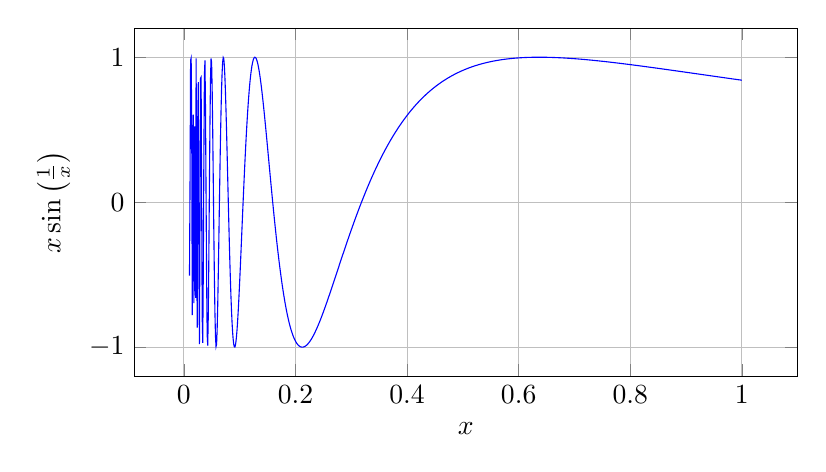
\begin{tikzpicture}
                    \begin{axis}[
                        domain=0.01:1, % 定义域
                        samples=1000, % 采样点数
                        xlabel=$x$,
                        ylabel={$x \sin\left(\frac{1}{x}\right)$},
                        grid=both,
                        width=10cm,
                        height=6cm
                    ]
                    \addplot[blue] {sin(deg(1/x))};
                    \end{axis}
                \end{tikzpicture}

                \begin{center}
                    图1. \(S=\{x\times\sin(\frac{1}{x})|0<x\leq1\}\)
                \end{center}
            \end{example}
            
            \begin{prf}
                不妨设\(f:[0,1]\to \cl S\)是连接\((0,0)\)点到\(\cl S\)中一点的道路.

                显然,存在\(\{x_n\},x_n\downarrow>0\),使\(f(x_n)=(-1)^n\neq0\)
                \[\because f(0)=0\]
                \[\therefore f\notin\Con([0,1],\cl S)\]
                \[Absurd!\]

                故\(\cl S\)不是道路连通的.
            \end{prf}

        \subsection{紧性}

            \begin{dfn}
                {紧集/Heine-Borel-Lebesgue性质}

                设拓扑空间$(S,\T)$, $S'\subset S$, 若$S'$的任何开覆盖均为有限子覆盖, 则$S'$为紧集. 
            \end{dfn}

            \begin{thm}
                []
                {}
                []
                []
                设\(T\)是\(S\)的一个子空间。那么,\(T\)是紧的当且仅当对于\(T\)中的每一个开覆盖,存在一个有限子集是\(T\)的开覆盖。
            \end{thm}
            
            \begin{prf}
                若\(T\)是紧致的,设\(\mathcal{A}'=\{A_{a}\} '\)是\(T\)由\(T\)中开集构成的一个开覆盖。选取合适的\(\{A_{a}\}\),有\(A_{a}'=A_{a}\cap T\)
            \end{prf}

            \begin{ppt}
                []
                {}
                []
                []
                Hausdorff空间的紧子集是闭的. 
                
                紧空间的闭子集是紧的.

                实直线上闭空间是紧致的。
            \end{ppt}
            
            \begin{ppt}
                []
                {}
                []
                []
                连续映射将紧集映射为紧集. 
            \end{ppt}

            注:以下内容我本来想放到第五章,不过为了Urysohn引理的完整性,还是放在前面来了。

            \begin{thm}
                {管状引理}
                [Tube Lemma]

                考虑积空间\(X\times Y\),其中\(Y\)是紧的。对于每一个包含\(x_0\times Y\)的开集\(N\),存在\(x_0\)的邻域\(U\),使得"管子"\(U\times Y\)被\(N\)包含。

                注意\(Y\)是紧的,若否,则管状引理不一定正确。如:取\(X=Y=\R,x_0=0,N=\{x\times y|\left|x\right|<\frac{1}{y^2+1}\}\)
                % \begin{figure}[h]
                %     \centering
                %     \begin{tikzpicture}
                %         \begin{axis}[
                %             domain=-1:1, % 定义域
                %             samples=1000, % 采样点数
                %             xlabel=$x$,
                %             ylabel=$y$,
                %             grid=both,
                %             width=10cm,
                %             height=6cm,
                %             restrict y to domain=-1:1,
                %             ytick={-1, -0.5, 0, 0.5, 1},
                %             xtick={-1, -0.5, 0, 0.5, 1}
                %         ]
                %         \addplot[blue, thick] gnuplot {1/(x**2+1)};
                %         \addplot[blue, thick] gnuplot {-1/(x**2+1)};
                %         \end{axis}
                %     \end{tikzpicture}
                % \end{figure}                
            \end{thm}

        \subsection{实直线上的紧致空间}
            
                

    \section{度量空间}
        
        \subsection{基本概念}
            
            \begin{dfn}
                {度量}
                [metric]

                设$S$为一个集合, 函数$d:S^2\to\R$称为是$S$上的一个\textbf{度量(Metric)/距离(Distance)}, 使得下列性质成立:

                (1)\[\forall x,y\in S, d(x,y)\geq0\]
                等号成立当且仅当$x=y$.

                (2)可交换性:
                \[\forall x,y\in X, d(x,y)=d(y,x).\]

                (3)三角不等式(Triangular Inequation):
                \[\forall x,y,z\in X, d(x,y)+d(y,z)\geq d(x,z)\]
            \end{dfn}
            
            \begin{dfn}
                {度量空间}[Metric Space]
                
            \end{dfn}

            \begin{dfn}
				{开球}
                [Open Ball]
				
				在度量空间中,包含一点x的开集,由与x的距离小于某个固定的正数r的一切点组成,这个开集称为以x为中心、r为半径的 \textbf{开球(Open Ball)},记作\(U_(x,r)\)或\(B_{r}(x)\)

				特别的, 在数轴上,我们称关于\(x\)对称的开区间\((x-\varepsilon,x+\varepsilon)\)为\(x\)的 \textbf{\(\varepsilon\)邻域(\(\varepsilon\)-Neighbourhood)},记作\(B_{\varepsilon}(x)\)或\(U_(x,\varepsilon)\)

				去心邻域记作\(U_(\dot{x},\varepsilon)\)
		\end{dfn}

        \subsection{分离定理}
            

\end{document}